\documentclass[11pt]{article}

\usepackage[T1]{fontenc}
\usepackage[margin=1in]{geometry}
\usepackage{amsmath,amssymb,amsthm,bm}
\usepackage{booktabs,array,tabularx}
\usepackage[dvipsnames]{xcolor}
\usepackage{graphicx}
\usepackage{microtype}
\usepackage{enumitem}
\usepackage[round,authoryear]{natbib}
\usepackage[hidelinks]{hyperref}
\setlength{\emergencystretch}{2em}
\Urlmuskip=0mu plus 1mu

\hypersetup{
  pdftitle={CADENCE: A prospective leakage-sealed test of cross-animal causal
  dynamical transfer},
  pdfauthor={Aarav Sinha}
}

\newtheorem{proposition}{Proposition}
\newtheorem{corollary}{Corollary}
\newcommand{\E}{\mathbb{E}}
\newcommand{\R}{\mathbb{R}}
\newcommand{\CS}{\operatorname{CS}}
\newcommand{\calS}{\mathcal{S}}
\newcommand{\calT}{\mathcal{T}}
\newcommand{\normal}{\mathrm{normal}}
\newcommand{\intervention}{\mathrm{int}}
\newcommand{\given}{\,\middle|\,}
\newcommand{\code}[1]{\texttt{#1}}
% Outcome-free manuscript helpers. These boxes are intentionally conspicuous:
% they must never be interpreted as an empirical result.
\newcommand{\NotEvaluated}{\textsc{not evaluated}}

\newcommand{\ProspectiveResultSlot}[2]{%
  \begin{center}
    \fcolorbox{BurntOrange}{BurntOrange!7}{%
      \parbox{0.92\linewidth}{%
        \textbf{\textcolor{BurntOrange}{Prospective result slot --- not
        populated.}} \textbf{#1}\par\smallskip
        #2\par\smallskip
        \emph{This box specifies planned reporting content. It contains no
        evaluation outcome and makes no performance claim. It may be replaced
        only from the immutable post-freeze aggregate and, for
        outcome-sequestered biological data, only after authorized unsealing,
        with failed and unevaluated gates retained verbatim.}%
      }%
    }
  \end{center}
}


\title{\textbf{CADENCE: A prospective, leakage-sealed test of\\
cross-animal causal dynamical transfer}}
\author{Aarav Sinha}
\date{Pre-outcome manuscript framework --- 25 July 2026}

\begin{document}
\maketitle

\begin{center}
  \fcolorbox{BrickRed}{BrickRed!7}{%
    \parbox{0.91\linewidth}{%
      \centering
      \textbf{\textcolor{BrickRed}{Pre-outcome status.}}
      This manuscript specifies a prospective analysis whose primary claim may
      fail. No public-seed teacher evaluation-world result, Allen
      evaluation-mouse response, or ICMS target response is reported here.
      Every empirical result slot is marked \NotEvaluated{} and must remain so
      until its predeclared post-freeze aggregation; outcome-sequestered
      biological cohorts additionally require authorized unsealing.
    }}
\end{center}

\begin{abstract}
Cross-animal alignment can reveal shared observational dynamics, but it does
not by itself show that a causal response operator transports to a new animal.
We introduce CADENCE, a hierarchical controlled state-space model and a
prospective test of a deliberately stronger claim: after an intervention
operator is learned from donor animals, can the complete neural and behavioral
response of a held-out animal be predicted when that animal contributes only
unperturbed activity? The model separates shared nonlinear normal flow, a
state-dependent low-rank intervention field, capacity-limited recording-adapter
residuals, adapter-specific observation maps, and a shared behavior readout. Its
stage-locked biological protocol physically separates target inputs from
target post-onset outcomes and hashes open-loop prediction bundles before a
single unsealing step. The primary biological test uses 28 sequestered mice from the
Allen Visual Behavior Ophys release; a six-mouse intracortical
microstimulation analysis is explicitly exploratory, with a randomized causal
contrast available in five mice. A public-seed procedural teacher benchmark
tests recoverability under known shared operators and supports a separate
impossibility construction, but is
ineligible for a headline conjunction. We state the latent
gauge invariance and the stronger observation-map non-identifiability that
arises when perturbations leave target normal support. Results will be
interpreted through a prespecified eight-part biological conjunction; failure
or missing evidence on any required component precludes the headline. This
version is a methods and analysis framework, not a report of evaluation
performance.
\end{abstract}

\section{Introduction}

Neural population recordings differ across animals in cell identity,
measurement geometry, and sampling, even when behavior and task structure are
shared. A substantial literature therefore aligns latent representations
across sessions and subjects, transfers decoders, or identifies conserved
population dynamics
\citep{chen2015srm,dyer2017cryptography,gallego2020stability,
safaie2023preserved,schneider2023cebra,gosztolai2025marble,jiang2025candy}.
Latent dynamical systems provide complementary machinery for smooth
single-trial inference, nonlinear generation, switching flow, and
behaviorally prioritized prediction
\citep{yu2009gpfa,pandarinath2018lfads,linderman2017rslds,
glaser2020multipop,sani2024dpad}. These achievements make cross-animal causal
prediction plausible; they do not establish it.

The distinction is consequential. An observational alignment can predict
where ordinary trajectories lie while being wrong about the vector field that
moves a trajectory after intervention. Conversely, an intervention operator
may be shared in a latent coordinate system while the target animal's neural
readout is underdetermined precisely where the intervention sends the state.
Perturbation is therefore not merely another test condition. It probes model
structure outside the information used to register a new animal
\citep{shenoy2021measurement,galgali2023residual}.

The closest adjacent biological result fits constrained cortical networks to
unperturbed activity and evaluates out-of-distribution optogenetic
inactivation \citep{sourmpis2026perturbations}. That work demonstrates why
normal fit is insufficient and why perturbation tests matter. Its in-vivo
perturbation endpoint is behavior, however, rather than a simultaneously
measured full neural response in a named held-out animal registered from
normal activity alone. CADENCE targets this narrower unresolved experiment.
It does not claim that intervention prediction, cross-animal alignment, or
neural dynamical modeling is itself new.

Our proposed contribution is conditional:

\begin{quote}
\emph{If every frozen gate passes, CADENCE will provide a leakage-free
demonstration that a donor-trained intervention operator can predict full
neural and primary-behavior trajectories in a held-out animal whose mapping
was learned only from normal activity.}
\end{quote}

``Unseen'' means unseen in the target animal. The intervention family and its
physical descriptor are observed in donors; globally novel intervention
classes are outside the claim. A positive sensory-omission result would not
establish transfer of direct neural control, and the small ICMS cohort remains
exploratory regardless of how favorable its evaluable predictive metrics are.

\begin{figure*}[t]
  \centering
  \setlength{\fboxsep}{4pt}
  \begin{tabular}{@{}c@{\hspace{2pt}}c@{\hspace{2pt}}c@{\hspace{2pt}}c
                    @{\hspace{2pt}}c@{\hspace{2pt}}c@{\hspace{2pt}}c
                    @{\hspace{2pt}}c@{\hspace{2pt}}c@{}}
    \fcolorbox{MidnightBlue}{MidnightBlue!5}{%
      \parbox[c][3.25cm][c]{0.13\textwidth}{\centering\scriptsize
      \textbf{1. Normal donors}\\[2pt]
      Fit shared flow \(F\), donor maps \(H_i\), behavior readout, and
      rank-two \(R_i\).}}
    &
    \(\boldsymbol{\longrightarrow}\)
    &
    \fcolorbox{MidnightBlue}{MidnightBlue!5}{%
      \parbox[c][3.25cm][c]{0.13\textwidth}{\centering\scriptsize
      \textbf{2. Donor interventions}\\[2pt]
      Freeze normal components; fit shared \(G\) and shrunk donor residuals.}}
    &
    \(\boldsymbol{\longrightarrow}\)
    &
    \fcolorbox{ForestGreen}{ForestGreen!6}{%
      \parbox[c][3.25cm][c]{0.13\textwidth}{\centering\scriptsize
      \textbf{3. New animal}\\[2pt]
      Fit its adapter using only \texttt{normal\_fit}; select on
      \texttt{normal\_val}.}}
    &
    \(\boldsymbol{\longrightarrow}\)
    &
    \fcolorbox{ForestGreen}{ForestGreen!6}{%
      \parbox[c][3.25cm][c]{0.13\textwidth}{\centering\scriptsize
      \textbf{4. Predict and hash}\\[2pt]
      Use the allowed dataset-specific initialization; persist SHA-256 before
      outcomes open.}}
    &
    \(\boldsymbol{\longrightarrow}\)
    &
    \fcolorbox{BurntOrange}{BurntOrange!7}{%
      \parbox[c][3.25cm][c]{0.13\textwidth}{\centering\scriptsize
      \textbf{5. Unseal once}\\[2pt]
      Verify hashes, mount post-onset outcomes, score all channels, and report
      the conjunction.}}
  \end{tabular}
  \caption{\textbf{The information boundary is part of the estimand.}
  Target-animal intervention outcomes cannot affect preprocessing, adaptation,
  early stopping, uncertainty calibration, or method selection.}
  \label{fig:protocol}
\end{figure*}


\section{Formal target of inference}
\label{sec:estimand}

\subsection{Units, information sets, and potential trajectories}

Let \(i\) index animals, \(q\) index eligible intervention queries, \(t\) index
post-onset time, and \(a\) denote an intervention descriptor. The multivariate
potential trajectory
\[
  Y_{iq}(t;a)
  =
  \bigl(
    Y^{\mathrm{neural}}_{iq1}(t;a),\ldots,
    Y^{\mathrm{neural}}_{iqp_i}(t;a),
    Y^{\mathrm{behavior}}_{iq}(t;a)
  \bigr)
\]
contains every prespecified neural channel and primary behavioral variable.
The target-animal effect is
\begin{equation}
  \tau_i(t,a)
  =
  \E_q\!\left[
    Y_{iq}(t;a)-Y_{iq}(t;0)
    \given i,\ q\text{ eligible}
  \right].
  \label{eq:estimand}
\end{equation}
The expectation is over the dataset-specific eligible risk set, not over a
hypothetical unrestricted intervention population.

For target animal \(i^\star\), fitting has access to donor normal and
intervention data and target normal support
\(\mathcal{D}_{i^\star}^{\normal}\). Prediction uses scheduled inputs,
intervention descriptors, and the dataset-specific initialization described
below. It has no access to
target post-onset neural activity, animal-generated action/choice, reward,
success label, or response time. Deterministic query construction may use only the predeclared,
allowed schedule, descriptor, and initialization; target intervention
outcomes may not enter fitted or response-dependent preprocessing,
normalization, channel selection, early stopping, hyperparameter selection, or
uncertainty calibration. The predicted causal trajectory is the difference
between treated and control open-loop rollouts from the same encoded
initialization:
\[
  \widehat{\tau}_{i^\star q}(t,a)
  =
  \widehat{Y}_{i^\star q}(t;a)
  -
  \widehat{Y}_{i^\star q}(t;0).
\]

The animal is the biological replication unit. Trials, cells, conditions,
sessions, time bins, and random optimization seeds are repeated measurements
within animal and cannot increase the inferential sample size. In the
procedural benchmark, the independently generated world is the unit: its four
targets are averaged equally before any bootstrap or sign-flip test. These
world-level intervals remain procedural and non-headline.

\subsection{Dataset-specific causal contrasts}

Allen omissions occur in an eligible expected-flash risk set. Within each
mouse, the omitted-flash trajectory is contrasted with a separate normal
effect-control pool. Controls are chosen without reading outcomes by the
frozen hierarchy: exact preceding image and flashes-since-change; image plus a
prespecified risk bin; image only; risk bin only; then the complete eligible
pool. Fallback and effective control counts are reported. The corresponding
estimand is therefore an eligible-risk-set omission effect, not an
unqualified effect of arbitrary visual removal.

For ICMS, each positive-current condition is contrasted within session and
trial block against randomized zero-current catches. Conditions are first
aggregated within session and sessions are then weighted equally within
animal. Five mice are design-eligible; the primary aggregate additionally
requires every prespecified session/condition to have validated same-block
catch support, or the five-mouse cohort is incomplete and \NotEvaluated{}.
ICMS83 has no
released catch trials; its guarded-ITI reference supports normal calibration
and a nonrandomized sensitivity, but it cannot enter the causal-skill
conjunction.

Allen and teacher rollouts start from each query's final pre-onset sample.
ICMS is a prespecified marginal condition--response exception: before target
stimulation metadata are opened, each session's predictions are averaged over
16 signal-blind normal-audit contexts on the full physical action lattice.
Scoring later interpolates those curves to realized descriptors and compares
condition means. ICMS therefore does not test trial-specific state
initialization.

\section{Model}
\label{sec:model}

\subsection{Hierarchical controlled dynamics}

CADENCE posits a latent state \(z_{it}\in\R^d\), scheduled task input \(u_{it}\),
and action vector \(a_{it}\). Here \(i\) indexes a recording adapter in the
model equations: an animal for teacher/Allen and an animal--session pair for
ICMS; inferential replication remains at the animal level.
\begin{align}
  z_{i,t+1}
    &= F_\theta(z_{it},u_{it})
       + R_i(z_{it})
       + G_\phi(z_{it})a_{it}
       + \delta_i(a_{it}),
       \label{eq:dynamics}\\
  y^{\mathrm{neural}}_{it}
    &= H_i^{\mathrm{neural}}(z_{it})+\epsilon^{y}_{it},\\
  y^{\mathrm{behavior}}_{it}
    &= A_i H^{\mathrm{behavior}}(z_{it})+b_i+\epsilon^{b}_{it}.
    \label{eq:observations}
\end{align}
The shared normal transition is a residual discretization
\[
  F_\theta(z,u)=z+\Delta\{-z+f_\theta([z,u])\}.
\]
The recording-adapter normal residual is capacity limited:
\[
  R_i(z)=\Delta\,U_iV_i\tanh(z),
  \qquad
  \operatorname{rank}(U_iV_i)\leq 2.
\]
For intervention channel \(c\), the implemented state-conditioned field is
\begin{equation}
  g_c(z)
  =
  \Delta\Bigl[
    b_c+L_cM_c\tanh(z)
  \Bigr],
  \qquad
  \operatorname{rank}(L_cM_c)\leq r_G,
  \label{eq:lowrankG}
\end{equation}
and \(G_\phi(z)a=\sum_c a_c g_c(z)\). The full teacher configuration uses
\(d=8\), \(r_G=2\), and \(\Delta=0.05\); full Allen uses
\(d=12\), \(r_G=2\), and \(\Delta=0.1\); and full ICMS uses
\(d=12\), \(r_G=4\), and \(\Delta=1/30\). All three use rank-two adapter
residuals. A shrunk additive donor term \(\delta_i\), grouped by animal,
captures residual intervention
heterogeneity. It is never estimated for a target: the point prediction uses
its donor-distribution mean of zero, while uncertainty draws integrate over
the donor distribution. Training-donor deltas are projected to exact zero mean
after every optimizer step, including after the final update.

Each recording adapter has an encoder, neural decoder, and affine behavior
calibration because recorded cells are not matched. The adapter is
animal-specific for teacher and Allen and session-specific (but nested within
animal) for ICMS. Donor intervention residuals remain grouped by animal.
Behavior otherwise uses a shared decoder. Neural and behavioral observations are
jointly encoded during normal-only adaptation; future target samples are never
teacher-forced into an intervention rollout.
For the teacher benchmark's primary neural endpoint, every learned method uses
a separate softplus-Poisson linear quasi-likelihood readout fit on frozen
open-loop target \(\normal\)-fit rollouts. Adam uses the frozen readout weight
decay of \(0.2\), and the additional explicit ridge coefficient is selected
only on \(\normal\)-validation rollouts. The model's native neural decoder is
retained as a separately labeled diagnostic, not silently substituted into the
primary teacher score.

\subsection{Stage-locked fitting}

The optimization stages instantiate the information boundary in
Figure~\ref{fig:protocol}:

\begin{enumerate}[leftmargin=*,label=\textbf{Stage \arabic*.}]
  \item Fit \(F_\theta\), the shared behavior decoder, donor observation maps,
    and donor \(R_i\) using normal donor sequences.
  \item Freeze normal components. Fit \(G_\phi\) and shrunk donor
    intervention residuals on training-donor perturbations, with whole-animal
    validation.
  \item Register target \(i^\star\). Fit its encoder, observation map, behavior
    calibration, and capacity-limited residual only on
    \(\mathcal{D}_{i^\star}^{\normal}\); select checkpoints using target
    normal validation.
  \item Freeze every parameter. For trial-conditional teacher and Allen
    queries, encode the final pre-onset sample; for ICMS, use the frozen
    normal-audit context ensemble. Roll out treated and control schedules open
    loop, then serialize and hash every prediction.
  \item Verify the hash and freeze attestation, mount the physically separate
    target outcomes once, and score.
\end{enumerate}

Locked preparation fsyncs an active-seal journal before changing target
permissions. Interrupted uncommitted artifacts are quarantined rather than
overwritten or deleted, and re-entry idempotently re-seals or restores the
target. The journal/registry is removed only after the score completion and a
separately hashed post-score restoration completion are durable.

Within each outer fold, candidate \(F\) is fit only on intervention-training
donors. The validation animal receives normal-only adapters with \(F\) frozen
and selects \(G\) epochs. A fresh model then refits \(F\) and \(G\) on all
outer donors for those fixed epoch counts before target adaptation.

Dataset-specific normal objectives use masked reconstruction, dynamics
consistency, variance-collapse control, and residual shrinkage. ICMS
additionally uses a variational KL term; teacher adds a short open-loop loss.
The intervention objective evaluates complete donor post-onset rollouts after
encoding only the last pre-onset sample. Architecture,
optimization budget, and all early-stopping data are fixed before sequestered
biological outcomes open.

\section{What is and is not identifiable}
\label{sec:identifiability}

The observed-space causal trajectory in Equation~\ref{eq:estimand}
is the scientific target. Absolute latent coordinates are not.

\begin{proposition}[Functional latent gauge invariance]
\label{prop:gauge}
Viewed as unrestricted functions, not necessarily within the implemented
factorized-\(\tanh\) parameter class, let
\(Q:\R^d\rightarrow\R^d\) be invertible and define
\(\widetilde z=Qz\). For any model \((F,G,R_i,\delta_i,H_i)\), define
\begin{align*}
  \widetilde F(\widetilde z,u)
    &= QF(Q^{-1}\widetilde z,u),&
  \widetilde G(\widetilde z)
    &= QG(Q^{-1}\widetilde z),\\
  \widetilde R_i(\widetilde z)
    &= QR_i(Q^{-1}\widetilde z),&
  \widetilde\delta_i(a)
    &= Q\delta_i(a),\\
  \widetilde H_i(\widetilde z)
    &= H_i(Q^{-1}\widetilde z).
\end{align*}
Then the transformed and original models induce identical observed normal and
intervention trajectories.
\end{proposition}

\begin{proof}
If \(\widetilde z_t=Qz_t\), substitution into the transformed transition gives
\(\widetilde z_{t+1}=Qz_{t+1}\) by induction. The transformed observation is
\(\widetilde H_i(\widetilde z_t)=H_i(z_t)\). Thus every likelihood and
observed-space causal effect is unchanged.
\end{proof}

Consequently, recovery of \(F\) or \(G\) in a particular coordinate system is
not meaningful without gauge alignment. Teacher diagnostics fit an affine
gauge using target \emph{normal-fit} states only; they remain diagnostics and
cannot substitute for observed neural and behavioral prediction.

Gauge freedom is benign because it leaves observations invariant. A more
serious ambiguity appears when the target observation map is learned only on
normal support.

\begin{proposition}[Normal-support non-identifiability]
\label{prop:support}
Let \(\calS_i\subset\R^d\) be the support of target normal latent states and let
\(\calT_i\) contain states visited after intervention. Suppose the observation
class contains two maps \(H_i\) and \(H_i'\) that agree on \(\calS_i\) but
differ at some \(z^\star\in\calT_i\). Then no procedure using donor data and
target normal data alone can identify the target observation at \(z^\star\).
\end{proposition}

\begin{proof}
The two maps induce exactly the same distribution for every target datum
available before unsealing, so any normal-only estimator has the same
distribution under both models. Yet their target intervention observations at
\(z^\star\) differ. Therefore the available information cannot distinguish
the two predictions.
\end{proof}

The ambiguity exists even for linear observation maps. If normal states span a
proper subspace \(S\subsetneq\R^d\), choose \(v\in S^\perp\) and any nonzero
output vector \(c\). Then
\[
  H_i'(z)=H_i(z)+cv^\top z
\]
agrees with \(H_i\) on all normal states but differs whenever an intervention
produces \(v^\top z\neq0\). Low rank in Equation~\ref{eq:lowrankG}
regularizes the intervention field but does not resolve this ambiguity: a
rank-one perturbation can still leave \(S\). Linear \(H_i\) becomes
estimable---within the shared gauge---only under adequate target normal
excitation; a nonlinear \(H_i\) additionally requires coverage or structural
regularity beyond the observed support.

\begin{corollary}[Impossibility pair]
\label{cor:impossibility}
Consider two worlds that have identical donor and target normal distributions
but opposite private target intervention effects, \(\tau\) and \(-\tau\). Any
normal-only target predictor \(p\) is identical in the two worlds, and its
average squared error across them is at least that of the zero-effect
predictor.
\end{corollary}

\begin{proof}
\[
  \tfrac12\{\lVert p-\tau\rVert^2+\lVert p+\tau\rVert^2\}
  =\lVert p\rVert^2+\lVert\tau\rVert^2
  \geq \lVert\tau\rVert^2.
\]
The final term is the zero-effect error in either world.
\end{proof}

The teacher benchmark implements this pair by making the target private
intervention direction independent of all normal data and flipping its sign.
A model should fail there. More generally, a negative neural result alongside
positive latent or behavioral diagnostics is compatible with
Proposition~\ref{prop:support}; it is not evidence that an
arbitrary observation map was actually recoverable.

\section{Evaluation resources}
\label{sec:data}

\begin{table}[t]
  \centering
  \caption{\textbf{Frozen evaluation resources.} Counts describe the
  prespecified inputs, not model performance. Sessions, trials, and cells are
  repeated measurements. Animals are the biological replication units; in the
  teacher benchmark, four targets are averaged within each independently
  generated world and the world is the inferential unit.}
  \label{tab:datasets}
  \small
  \begin{tabularx}{\linewidth}{@{}
    >{\raggedright\arraybackslash}p{0.19\linewidth}
    >{\raggedright\arraybackslash}p{0.23\linewidth}
    >{\raggedright\arraybackslash}X@{}}
    \toprule
    Resource & Independent units & Frozen scope \\
    \midrule
    Teacher RNN
      & 10 development and 20 public-seed procedural evaluation worlds;
        4 nested targets per world
      & Known nonlinear dynamics, six intervention channels, variable
        64--128-neuron maps, paired counterfactual twins, and an explicit
        non-identifiability pair. Internal \code{locked} label is retained
        only for schema compatibility. \\
    Allen Visual Behavior Ophys 1.1.0
      & 32 mice: 4 development and 28 locked evaluation mice
      & VISp, Slc17a7-IRES2-Cre, 175~\(\mu\)m, familiar active sessions;
        6,768 cells, 65,522 clean normal windows, and 4,707 eligible omission
        windows. \\
    DANDI:001868 v0.260715.2016
      & 6 task mice; randomized causal contrast in 5
      & 45 trimodal source sessions (v1 scores spikes and wheel); 14,734
        canonical 100-Hz, 70-pulse trials;
        1,400 randomized catches and 932 signal-blind guarded-ITI calibration
        windows. ICMS83 is absolute-trajectory-only. \\
    \bottomrule
  \end{tabularx}
\end{table}


\subsection{Procedural teacher RNN}

The teacher generator fixes a nonlinear contractive normal operator,
state-dependent rank-two intervention fields, exact rank-two animal residuals,
animal-specific 64--128-neuron observation maps, three behaviors, and
negative-binomial neural noise. Each intervention trial has a counterfactual
twin with the same initial state, task drive, process innovations, and
observation-noise variables. Ten worlds are reserved for development and 20
for a predeclared deterministic post-freeze procedural evaluation, with four
nested targets per world. All 20 numeric evaluation seeds are public plaintext
in \code{configs/teacher.yaml}; no seed secrecy, outcome blinding, or
sequestration is claimed. The internal partition label \code{locked} is
retained only for schema compatibility. These 30 default seed worlds
instantiate the frozen main regime; they do not silently vary stress axes.
Target metrics are averaged equally within world, leaving \(n=20\)
independent units for procedural intervals. Those intervals are descriptive
and can never enter a biological or headline conjunction. Separately, the
generator supports explicit diagnostic stress settings for conserved
intervention strength, animal residual strength, donor support, target
population size, normal-state coverage, and the impossibility construction in
Corollary~\ref{cor:impossibility}. Semantically addressed random streams
ensure that explicitly adding such a setting does not alter unrelated
examples.

\subsection{Allen Visual Behavior Ophys}

The primary biological cohort is frozen from the Allen Visual Behavior Ophys
1.1.0 release \citep{allenVBOrelease}: one familiar active VISp experiment per
Slc17a7-IRES2-Cre mouse
at 175~\(\mu\)m, with at least 40 cells. Four mice selected by a deterministic
hash rule are development-only; 28 mice remain in five locked outer folds.
The full \([-1,2]\)-s window must have common neural, running, pupil, and lick
support. Normal anchors are active ordinary presentations, at least 3~s from
an omission, change, or sham. A deterministic 160-window adapter pool is split
70/15/15\% into normal fit, validation, and audit sets; every remaining clean
normal forms a separate effect-control pool. The primary outcomes over
\(0\)--2~s are every prespecified cell's event-rate trajectory and running
speed. Pupil area and lick rate are secondary and cannot rescue a failed
running gate.

\subsection{DANDI:001868 ICMS}

The exploratory direct-intervention analysis uses the immutable published
DANDI:001868 version 0.260715.2016
\citep{kim2026dandi001868,kim2026learning,kim2026acceptedrecord}. Six task mice contribute 45
sessions containing behavior, ephys, and ophys. Each leave-one-animal-out fold
uses one rotating whole-animal validation donor. Target normal calibration
combines zero-current catches with signal-blind ITI windows selected from the
complement of all trial and stimulation intervals after a 2-s guard on both
sides. No pre-stimulation fragment of a target intervention trial is
relabelled as normal.
The source-authored \code{is\_good\_trial} flag is an additional prespecified
signal-support restriction applied before neural or wheel signals are read.
Its released NWB description defines \code{true} as matching two-photon
coverage of the stimulation window, \code{false} as no overlapping imaging
frames, and defaults to \code{true} when no source MAT key exists. It is not a
hit/response filter and is not used for tuning; the ICMS estimand is explicitly
conditional on this released cross-modal-coverage flag.

The primary intervention family is the canonical 100-Hz, 70-pulse,
167-\(\mu\)s train (approximately 0.7~s). Longer or otherwise noncanonical
recorded trains are outside the frozen query lattice and labeled
\code{OUT\_OF\_SCOPE\_NOT\_SCORED}; their analysis is \NotEvaluated{}, not a
duration-generalization sensitivity. Actions use physical current, pulse
physics, and electrode coordinates rather than implant-specific raw channel
identifiers. The primary neural endpoint is curated sorted-unit activity with
a conservative 2-ms pre-train through 5-ms post-train exclusion. Frozen v1
processed files do not retain a distinct unmasked full-train spike tensor, so
the full-train spike analysis is \NotEvaluated{}. All source sessions include
ephys, ophys, and wheel data, but frozen v1 models and scores use sorted spikes
and wheel only. Sparse volumetric z-stack observations remain in processed
files for a future native-mask analysis and are \NotEvaluated{} here; they are
not described as a simultaneous 30-Hz population.

ICMS responses can depend on current, distance, direct axonal recruitment, and
transsynaptic dynamics
\citep{stoney1968extent,tehovnik2006direct,butovas2003spatiotemporal,
histed2009direct,lycke2023ultraflexible}. This biology motivates a physical
action descriptor and cautions against interpreting stimulation as one generic
binary input.

\section{Scores, uncertainty, and decision rule}
\label{sec:evaluation}

\subsection{Full-trajectory scores}

For target \(i\), let \(s_{ik}\) be a channel scale estimated exclusively from
that animal's normal-fit support, and let \(m_{iqtk}\) be the fixed observation
mask. Causal skill is
\begin{equation}
  \CS_i
  =
  1-
  \frac{
    \sum_{q,t,k}m_{iqtk}
      \left[
      \{\widehat{\tau}_{iqtk}-\tau_{iqtk}\}/s_{ik}
      \right]^2
  }{
    \sum_{q,t,k}m_{iqtk}
      \left(\tau_{iqtk}/s_{ik}\right)^2
  }.
  \label{eq:skill}
\end{equation}
A perfect prediction scores 1, prediction of no causal effect scores 0, and a
negative value is worse than no effect. Every retained time--channel element
is scored; responsive-cell selection is forbidden. Scores are first computed
within animal and then averaged with equal animal weight.
The scale \(s_{ik}\) is the sample standard deviation on target normal-fit
support, clipped to the within-animal 10th--90th percentiles of positive,
finite channel standard deviations. A zero-effect-energy stratum has undefined
skill; it is retained in the stratum ledger but excluded from the finite-stratum
mean.

Allen's frozen primary is a dataset-specific exception to the pooled ratio in
Equation~\ref{eq:skill}. Within each mouse, predicted and observed effects are
first averaged within every eligible image identity \(\times\) risk bin
\(\times\) matching-fallback stratum. Causal skill is computed separately in
each stratum and then averaged across strata. The ratio pooled over all
query--time--channel elements is retained only as a secondary Allen summary.

Frozen v1 emits normalized trajectory RMSE and selected time-resolved
observed-space summaries. It does not emit response-summary or split-half
reliability-ceiling artifacts; those fields remain \NotEvaluated{}.
Absolute-trajectory error is secondary because shared baseline activity can
make a failed effect prediction look accurate.
A positive claim requires posterior trajectory draws evaluated by the
multivariate energy score, which is proper and lower-is-better. If a runner
does not emit valid draws and this score, the proper-score gate remains
\NotEvaluated{}.

\subsection{Comparators and ablations}

Dataset-specific frozen matrices give methods the same allowed target-normal
support and descriptors. Learned methods share the encoded initialization;
fixed templates use the frozen matched-normal control. All matrices include
CADENCE plus linear, additive, and black-box learned methods with the same
latent and hidden dimensions. No-effect, condition--time, and nearest-donor
comparators are included where defined. Allen additionally includes a
cell-functional ridge atlas and two CADENCE ablations. Teacher uses its
separately listed native-decoder and adaptation/residual diagnostics. Frozen
ICMS v1 emits no CADENCE ablations; a criterion requiring one would remain
\NotEvaluated{}. A learned pooled neural model without animal maps is
unavailable because heterogeneous neuron counts do not define a common output
dimension. Evaluation-only oracles are excluded from the baseline envelope. The reporting
layer constructs a separate post-outcome envelope for each target and endpoint:
the maximum observed score over \emph{all} eligible non-oracle comparators and
ablations. This deliberately conservative reference is not a
validation-selected single baseline and is not a deployable model-selection
rule.

\subsection{Uncertainty and animal-level inference}

A positive claim requires predictive uncertainty that integrates
donor-bootstrap ensembles, bootstraps of target normal support, donor
intervention random effects, and process variability estimated without target
interventions. It also requires split-conformal calibration using whole-animal
cases disjoint from fitting, early stopping, and model selection (or an
equivalent predeclared cross-fitted construction). Maximum standardized
trajectory residuals form a simultaneous 90\% band, with pointwise coverage,
whole-trajectory coverage, and width retained. The 95\% lower bound for
whole-trajectory coverage is the exact one-sided binomial bound across
independent animals, not a percentile bootstrap over binary indicators. In
particular, \(5/5\) covered ICMS animals cannot certify a lower bound of 0.80.
A runner that omits the required draws, disjoint calibration provenance, bands,
or coverage fields cannot satisfy the corresponding gate; reporting fails
closed to \NotEvaluated{}.

The primary mean and gain intervals are 95\% nonparametric bootstraps over
animals (20,000 resamples). Paired animal-level sign-flip tests are exhaustive;
sessions, trials, and neurons are never permuted as if independent animals.
For the teacher benchmark, four targets are first averaged within world and
the 20 worlds are bootstrapped or sign-flipped. These intervals are procedural
only; the teacher conjunction remains \NotEvaluated{}. Duplicating targets
within a world cannot tighten inference. Incomplete biological headline
cohorts cannot evaluate a gate.

\subsection{Falsification and leakage audits}

Gate 6 jointly requires four exact paired animal-level sign-flip tests
(neural and behavior skill above zero, and neural and behavior gain above
zero) plus three explicit randomization controls: target-label permutation,
donor intervention-semantic shuffle, and animal-adapter shuffle. Gate 8
consumes pseudo-onsets on normal trials and a pre-onset effect check.
Each randomization control retains its frozen procedure, test value, and
artifact. Its canonical relative filename and observed digest must be bound
into the runner's authenticated completion chain; a bare pass flag or claimed
digest is insufficient. Each negative control
retains an equivalence margin and confidence interval whose bounds must lie
inside that margin.
Failure to reject a conventional null is not silently treated as evidence of
equivalence: pre-onset and pseudo-onset controls require their explicit null
criteria. A runner that omits a required diagnostic leaves the associated gate
\NotEvaluated{}. Onset shifts, initial-state-only decoding, and the teacher
impossibility pair are additional diagnostics but are not silently counted as
one of the declared gate inputs; frozen v1 does not emit all of them. Sentinel
invariance is an executable leakage test rather than a biological null. A
changed prediction hash, a target intervention row in a
fitted transform, or a sealed sentinel reaching a trainable module invalidates
the fold.

\subsection{Conjunctive headline}

\begin{table}[t]
  \centering
  \caption{\textbf{Pre-outcome conjunction ledger.} The statuses below are
  intentionally fixed to \NotEvaluated{} until complete frozen cohorts are
  scored. A single failed gate defeats the corresponding dataset-level
  headline. The teacher benchmark is reported separately and cannot establish
  a biological claim; its public seeds make it ineligible for this
  conjunction.}
  \label{tab:gates}
  \footnotesize
  \begin{tabularx}{\linewidth}{@{}cXcc@{}}
    \toprule
    Gate & Frozen criterion & Allen & ICMS \\
    \midrule
    1 & Randomized manipulation has nonzero neural and primary-behavior
        effects. & \NotEvaluated & \NotEvaluated \\
    2 & Equal-animal 95\% CI for neural causal skill lies above zero.
        & \NotEvaluated & \NotEvaluated \\
    3 & Equal-animal 95\% CI for primary-behavior causal skill lies above zero.
        & \NotEvaluated & \NotEvaluated \\
    4 & Mean gain is at least 0.10 over the per-target post-outcome envelope
        of all eligible non-oracle comparators and ablations for both
        endpoints, and both gain CIs lie above zero.
        & \NotEvaluated & \NotEvaluated \\
    5 & State-conditioned prediction improves proper score over the donor
        condition--time template. & \NotEvaluated & \NotEvaluated \\
    6 & Four exact paired animal-level sign-flip tests and all three declared
        animal/action randomization controls reject their nulls.
        & \NotEvaluated & \NotEvaluated \\
    7 & The 90\% simultaneous bands have an exact one-sided 95\% binomial
        coverage lower bound of at least 0.80 across animals.
        & \NotEvaluated & \NotEvaluated \\
    8 & Pre-onset and pseudo-onset controls satisfy their explicit null checks.
        & \NotEvaluated & \NotEvaluated \\
    \bottomrule
  \end{tabularx}
\end{table}


For an eligible biological dataset, the overall status is \textsc{pass} only
when all eight rows pass.
\textsc{Fail} is retained even if another row is missing; otherwise any missing
component yields \NotEvaluated{}. Allen development mice never enter the
headline. ICMS83 never enters its randomized causal summary. Teacher results
test recoverability under known assumptions but cannot establish a biological
shared operator. Because the teacher seeds are public, reporting fixes its
headline conjunction to \NotEvaluated{} regardless of numerical completeness.
Frozen v1 is fail-closed: its current biological runners do not emit everything
needed to pass Gate~1 or Gates~5--8. Missing components remain
\NotEvaluated{}, while an authenticated evaluated subcomponent that
contradicts a composite gate can still make that gate \textsc{fail}. This
release can therefore return \textsc{fail}, but it cannot return a biological
\textsc{pass}. Missing evidence cannot be retrofitted after unsealing.

\section{Pre-outcome development record}

The development sandbox is reported only to disclose method selection and the
known risk, not as confirmatory evidence. After removing validation-animal
normal leakage, ten teacher smoke worlds gave proposed condition-averaged
neural skill mean \(0.00173\), median \(0.0131\), range
\([-0.1175,0.0623]\), and 8/10 positive worlds. Proposed neural pathwise skill
had mean \(0.00878\) and was positive in 7/10. Behavior skill was positive in
10/10 (mean \(0.5049\)), whereas latent-effect skill was positive in 7/10
(mean \(0.1270\)). The evaluation-only gauge-plus-true-observation diagnostic
had mean neural skill \(0.0278\). On average, 9.79\% of readout query
coordinates fell outside the coordinate-wise range of target normal
rollouts. This mixed, near-zero neural result does not establish reliable
latent, operator, or observation-map transfer; it exposes estimation failure
and a measurable off-range burden consistent with, but not diagnostic of,
off-support extrapolation. Across the four allowed Allen development mice,
proposed neural causal skill had mean \(-8.63\times10^{-5}\), range
\([-1.85\times10^{-4},1.61\times10^{-7}]\), and 1/4 positive mice.
Proposed running causal skill had mean \(-4.91\times10^{-4}\), range
\([-1.69\times10^{-3},1.94\times10^{-4}]\), and 2/4 positive mice.
Thus neither Allen endpoint established transfer.

\begin{figure}[t]
  \centering
  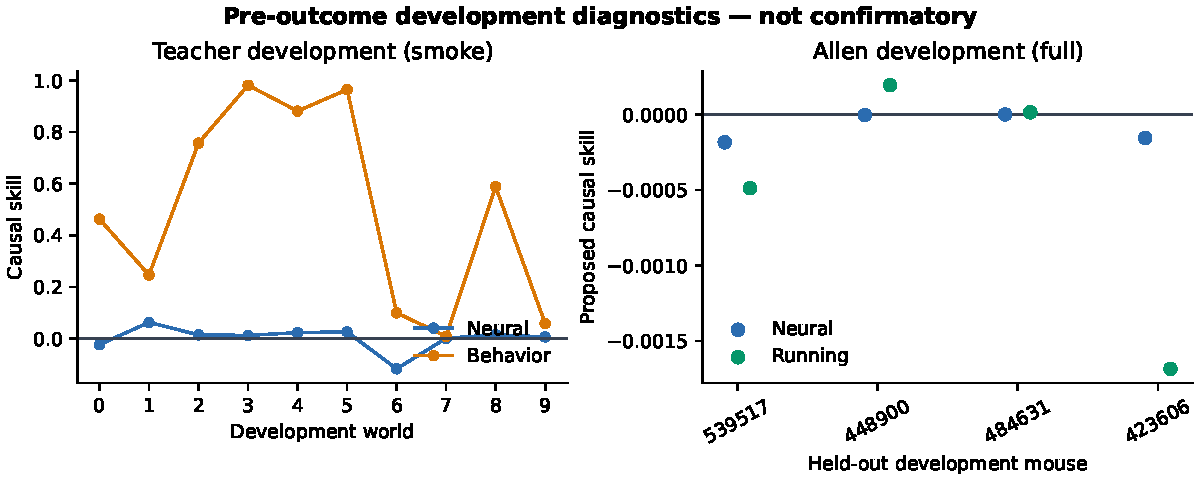
\includegraphics[width=\linewidth]{figures/development_diagnostics.pdf}
  \caption{\textbf{Authenticated pre-outcome development diagnostics.}
  Left: proposed condition-averaged neural and behavior causal skill in the
  ten teacher smoke worlds. Right: proposed neural and running causal skill
  in the four permitted Allen full-development mice. These observations
  disclose method-selection risk and are not confirmatory evidence.}
  \label{fig:development}
\end{figure}

No held-out ICMS stimulation outcome was used for model selection. A
pre-freeze schema regression did load one ICMS83 example container to verify
exceptional channel wiring, dimensions, catch count, and normal-ITI validity;
it did not print, score, summarize, or tune against a response trajectory.
ICMS83 is catch-free and excluded from the randomized causal cohort, and none
of the five randomized-effect mice was opened. These observations and accesses
were recorded before procedural evaluation outputs were run or randomized
biological outcomes were unsealed. They cannot be overwritten by choosing a
new architecture after seeing evaluation outcomes.

\section{Prospective results}
\label{sec:results}

\ProspectiveResultSlot{Teacher predeclared procedural evaluation (public
seed; non-headline).}{
Insert all 80 target predictions, nested four per each of 20 independent
deterministic post-freeze worlds; average targets within world before
inference. Report observed-space condition-averaged neural and behavioral
skills; realized-path diagnostics; latent/operator recovery only after a
normal-fit gauge; any separately instantiated diagnostic stress slices;
impossibility-pair behavior only if separately instantiated (otherwise
\NotEvaluated{}); all baselines; and a complete audit. Disclose the
public seeds, state explicitly whether neural observation-map transfer
succeeds, and retain the conjunction as \NotEvaluated{}.}

\ProspectiveResultSlot{Allen primary evaluation.}{
Insert one row per each of the 28 evaluation mice and the equal-animal
aggregate. Report neural event-rate and running causal skill first, strongest
baseline envelopes and uncertainty next, then pupil/lick secondary analyses,
matching fallback distributions, proper scores, coverage, falsifications, and
all eight gate statuses. Do not use secondary behavior to rescue running.}

\ProspectiveResultSlot{ICMS exploratory direct intervention.}{
Insert all six absolute-trajectory results, but restrict the randomized causal
aggregate to ICMS92, ICMS93, ICMS98, ICMS100, and ICMS101 and label \(n=5\).
Report primary artifact-robust sorted-spike and wheel trajectories, physical
current/site strata, uncertainty, and every unevaluated field. Keep
longer/noncanonical train rows \code{OUT\_OF\_SCOPE\_NOT\_SCORED} and their
analysis \NotEvaluated{}; do not score them as a frozen-v1 sensitivity.
Explicitly retain full-train spike and sparse-calcium analyses as
\NotEvaluated{} in frozen v1.
ICMS83 must remain absolute-only.}

\ProspectiveResultSlot{Conjunction and claim sentence.}{
Insert the machine-generated conjunction table without manual relabeling.
Write a positive claim only for a dataset whose eight gates all pass. If a
required gate fails, lead with the failure. If no gate fails but required
evidence is missing, use ``not evaluated,'' not ``passed'' or ``inconclusive
success.''}

\section{Interpretation}

The frozen design supports three qualitatively different outcomes. First,
positive neural and behavioral transfer with calibrated uncertainty would
support a shared operator over the measured animal, state-support, and
intervention family. It would not imply globally novel-action generalization
or universal neural coordinates. Second, transferable behavior but failed
cell-resolved neural prediction would be consistent with a shared coarse
latent effect whose target observation map is non-identifiable off normal
support. Third, failure already in latent or behavioral teacher endpoints
would implicate dynamics/operator estimation rather than only the biological
observation map.

Negative evidence is scientifically informative here. A model can reconstruct
normal data, align animals, and even recover a donor perturbation field while
failing the target response. Such a result limits what observational
cross-animal alignment licenses us to infer. The protocol therefore commits to
publishing failed and unevaluated gates rather than treating the locked cohort
as a second development set.

\section{Limitations}

\begin{enumerate}[leftmargin=*]
  \item \textbf{Identifiability is assumption-dependent.} Low-rank structure,
    donor conservation, and normal-state coverage are inductive biases, not
    proofs that a target observation map extrapolates correctly.
  \item \textbf{Interventions are not globally novel.} The target action is
    unseen in that animal but represented in donors. Extrapolation to a new
    action class remains untested.
  \item \textbf{Allen scope is narrow.} The primary cohort is one cortical
    area, excitatory cell class, depth, task familiarity, and omission family.
    Matching estimates an eligible-risk-set effect and does not create paired
    counterfactuals.
  \item \textbf{ICMS is small and exploratory.} Only five animals support the
    randomized causal contrast; ICMS83 is nonrandomized for effects. The
    associated bioRxiv v1 manuscript is accepted at \emph{Science Advances},
    but no version-of-record DOI was located as of 2026-07-25; stimulation
    artifact, longitudinal learning, and implant geometry limit transport.
  \item \textbf{Modalities differ in support.} Sorted spikes are primary for
    ICMS. Volumetric calcium is sparsely observed by z-plane and cannot be
    interpreted as a simultaneous 30-Hz population.
  \item \textbf{Open-loop error compounds.} Long-horizon failures can combine
    initialization, normal-flow, intervention-field, and observation-map
    error. Oracle diagnostics localize failure but are not eligible evidence.
  \item \textbf{Uncertainty can remain underpowered.} Animal-level inference
    correctly exposes rather than hides the small biological sample,
    particularly for ICMS.
\end{enumerate}

\section{Reproducibility, data governance, and ethics}

Raw public datasets are excluded from version control; committed manifests
record immutable versions, asset identifiers, byte counts, and content hashes.
Locked profiles require a clean checkout at the exact annotated
\code{pre-outcome-v1.0.0} tag. Predictions and outcome bundles are physically
separate, and every prediction archive receives a SHA-256 digest before
scoring. Complete frozen aggregation uses the predeclared 20,000-resample seed
and runs only from the clean tagged reporter; locked input paths and SHA-256
digests are retained. The final machine-readable summary, long-form CSV,
compact \LaTeX{} table, and conjunction ledger are published atomically into a
new append-only directory with artifact sidecars and a completion manifest.
Missing uncertainty, coverage, or falsification fields remain
\NotEvaluated{}.

This project performs secondary analysis of public animal datasets and a
procedural simulation; it introduces no new animal experiment. Ethical and
regulatory approvals for data acquisition are documented by the source
studies. Reuse is subject to the source licenses and requires citation of the
Allen release and DANDI:001868.

\section{Conclusion}

CADENCE is a prospective biological falsification test, not a guarantee that causal
dynamics transfer across animals. Its scientific value rests on a strict
information boundary, observed-space endpoints, animal-level replication, and
a decision rule that is allowed to fail. The latent gauge is harmless for
observed prediction; extrapolation of a target neural map beyond normal support
is not. The frozen biological evaluations and public-seed procedural teacher
audit will determine whether the imposed structure is sufficient in their
declared scopes. Until then, the primary biological claim remains prospective.

\bibliographystyle{plainnat}
\bibliography{references}

\end{document}
